\documentclass[11pt]{article}
\usepackage{listings}
\usepackage{xcolor}
\usepackage{multirow}
\usepackage{multicol}
\usepackage{xparse}
\usepackage{amsmath}
\usepackage[BoldFont]{xeCJK}
\usepackage[most]{tcolorbox}
\usepackage[T1]{fontenc}

\usepackage{lmodern}

\graphicspath{ {./image/} }
\renewcommand\thesection{Question \ \arabic{section}}
\renewcommand\thesubsection{\arabic{section}-(\alph{subsection})}
\usepackage{hyperref}
\hypersetup{
    colorlinks=true,
    linkcolor=blue,
    filecolor=magenta,      
    urlcolor=cyan,
    pdftitle={習題5 },
    pdfpagemode=FullScreen,
}
\usepackage[a4paper, margin={3cm}]{geometry}
\linespread{1.15}
\lstset{language=C,keywordstyle={\bfseries \color{blue}}}
	

\title{習題5 \\\Large 總體經濟學原理與實習}
\author{B10703033\ 財金一\ 邱奕璉
\\ B10703103\ 財金一\ 許羽婷
\\ B10705007\ 資管一\ 劉冠甫
\\ B10705047\ 資管一\ 邱秉辰}
\date{April 1, 2022}

\setlength{\parindent}{0em}
\setlength{\parskip}{0.5em}

\setCJKmainfont{GenRyuMin TW}
\begin{document}



\maketitle

\section{}
\begin{figure}[h]
    \centering
    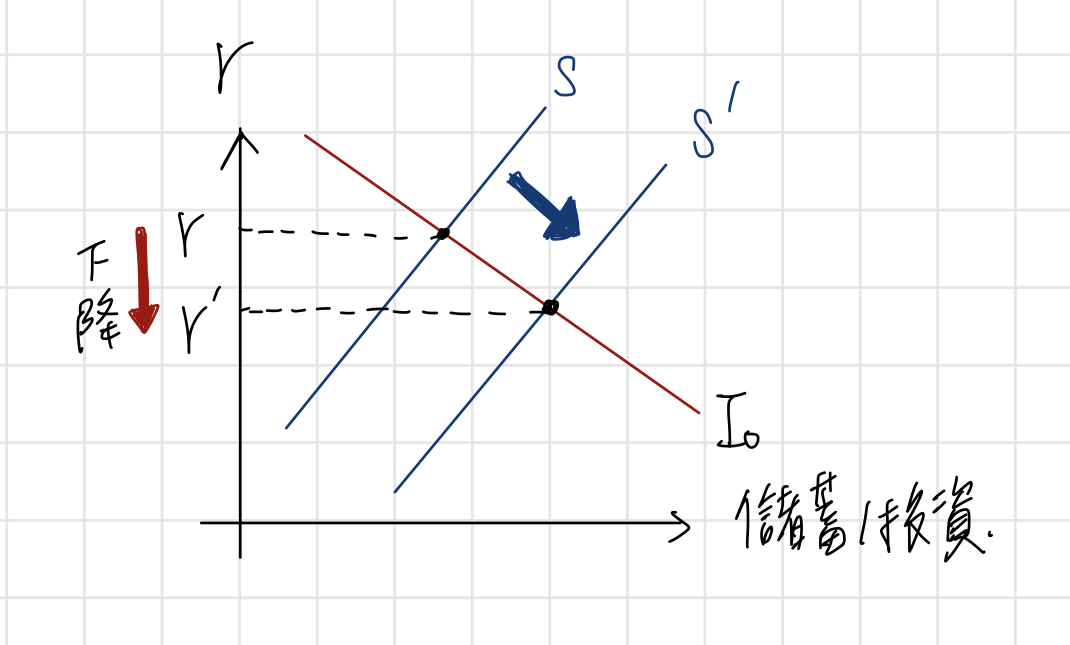
\includegraphics[scale = 0.3]{1.jpeg}
\end{figure}
全球儲蓄過剩造成可貸資金供給增加，導致供給線右移，使均衡利率下降。

\section{}
\subsection{}
$$
\frac{b_1}{p_1} = y_1-c_1-i_1
$$
\begin{itemize}
    \item 甲：$20 - 20 - 4 = -4$ （單位）$\implies$ 甲借入 4 單位
    \item 乙：$15 - 15 - 1 = -1$ （單位）$\implies$ 乙借入 1 單位
\end{itemize}
\subsection{}
$$
\frac{b_1}{p_1} = y_1-c_1-i_1
$$
\begin{itemize}
    \item 甲：$22 - 18 - 3 = 1$ （單位）
    \item 乙：$17 - 14 - 0 = 3$ （單位）
\end{itemize}

\subsection{}
\begin{figure}[h]
    \centering
    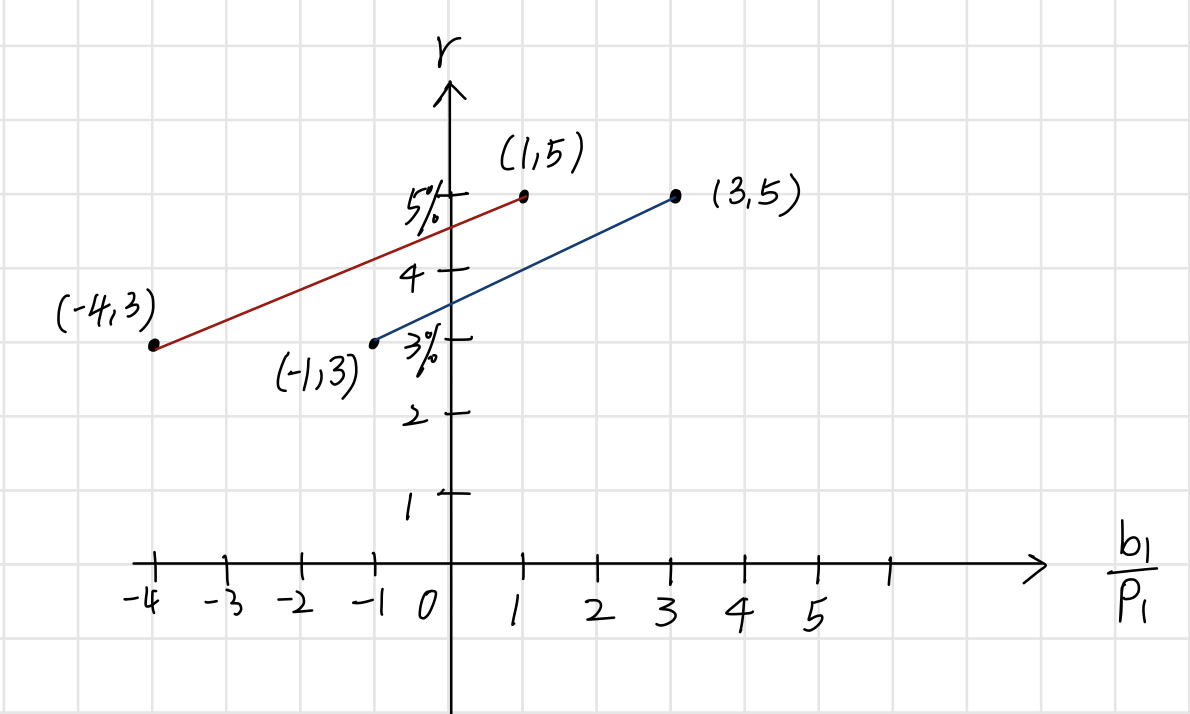
\includegraphics[scale = 0.3]{2c.jpeg}
\end{figure}

\subsection{}
\begin{figure}[h]
    \centering
    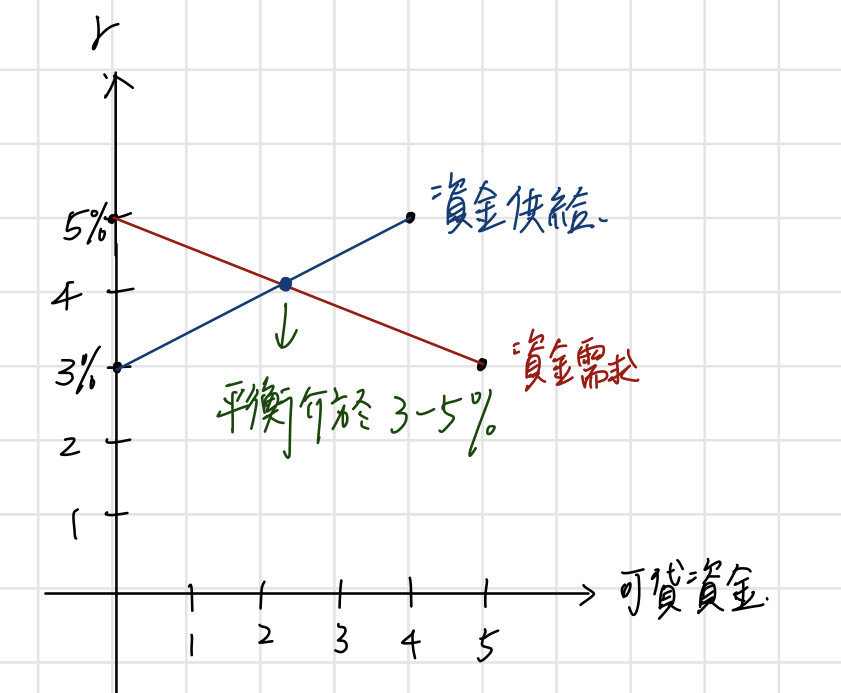
\includegraphics[scale = 0.32]{2d.jpeg}
\end{figure}
\begin{itemize}
    \item 實質利率為 5\% 時：總和供給為 4（單位）
    \item 實質利率為 3\% 時：總合需求為 5（單位）
\end{itemize}
\subsection{}
介於 3 至 5\%之間
\subsection{}
\begin{itemize}
    \item 利率為 3\% 時
    \begin{itemize}
        \item 總和儲蓄：0 + 0 = 0
        \item 總和投資：4 + 1 = 5
    \end{itemize}
    \item 利率為 5\% 時
    \begin{itemize}
        \item 總和儲蓄：4 + 3 = 7
        \item 總和投資：3 + 0 = 3
    \end{itemize}
\end{itemize}
\begin{figure}[h]
    \centering
    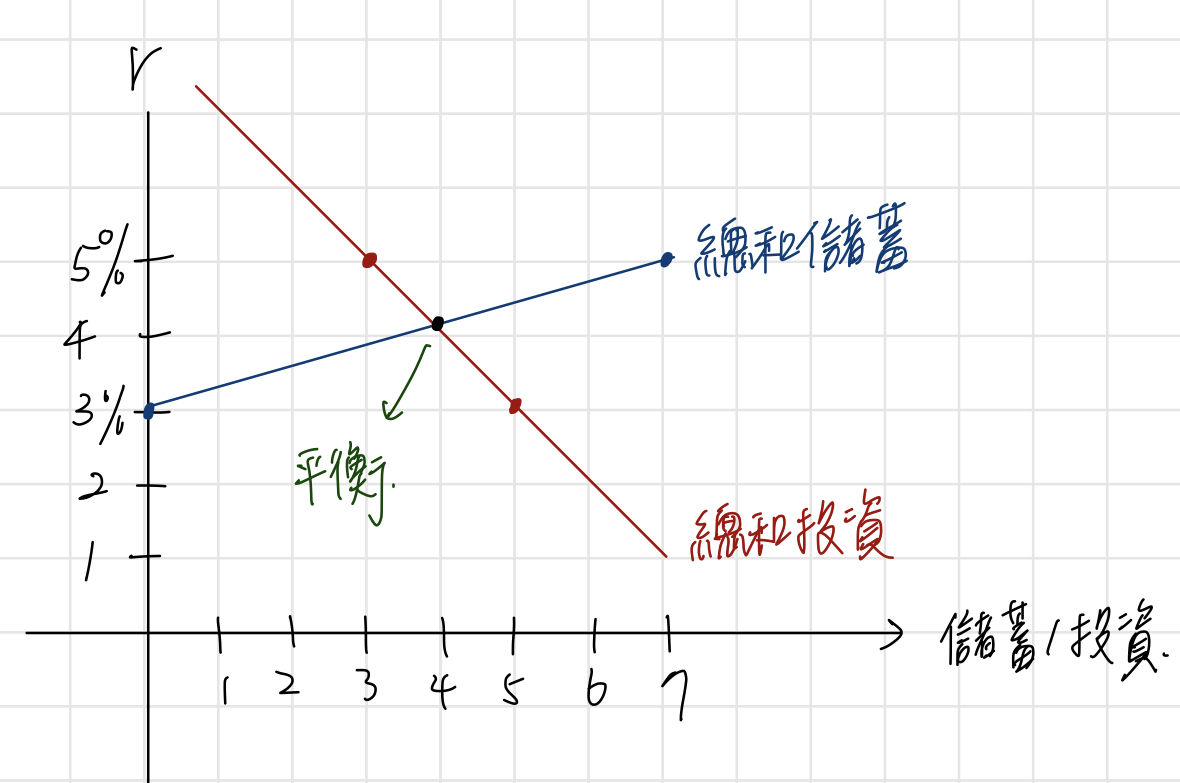
\includegraphics[scale = 0.3]{2e.jpeg}
\end{figure}

\subsection{}
大於 0 ，由 2(f)之圖表判斷出，當總和儲蓄等於總和投資時達到平衡，而此時平衡的金額為正。

\section{}
\subsection{}
\begin{figure}[h]
    \centering
    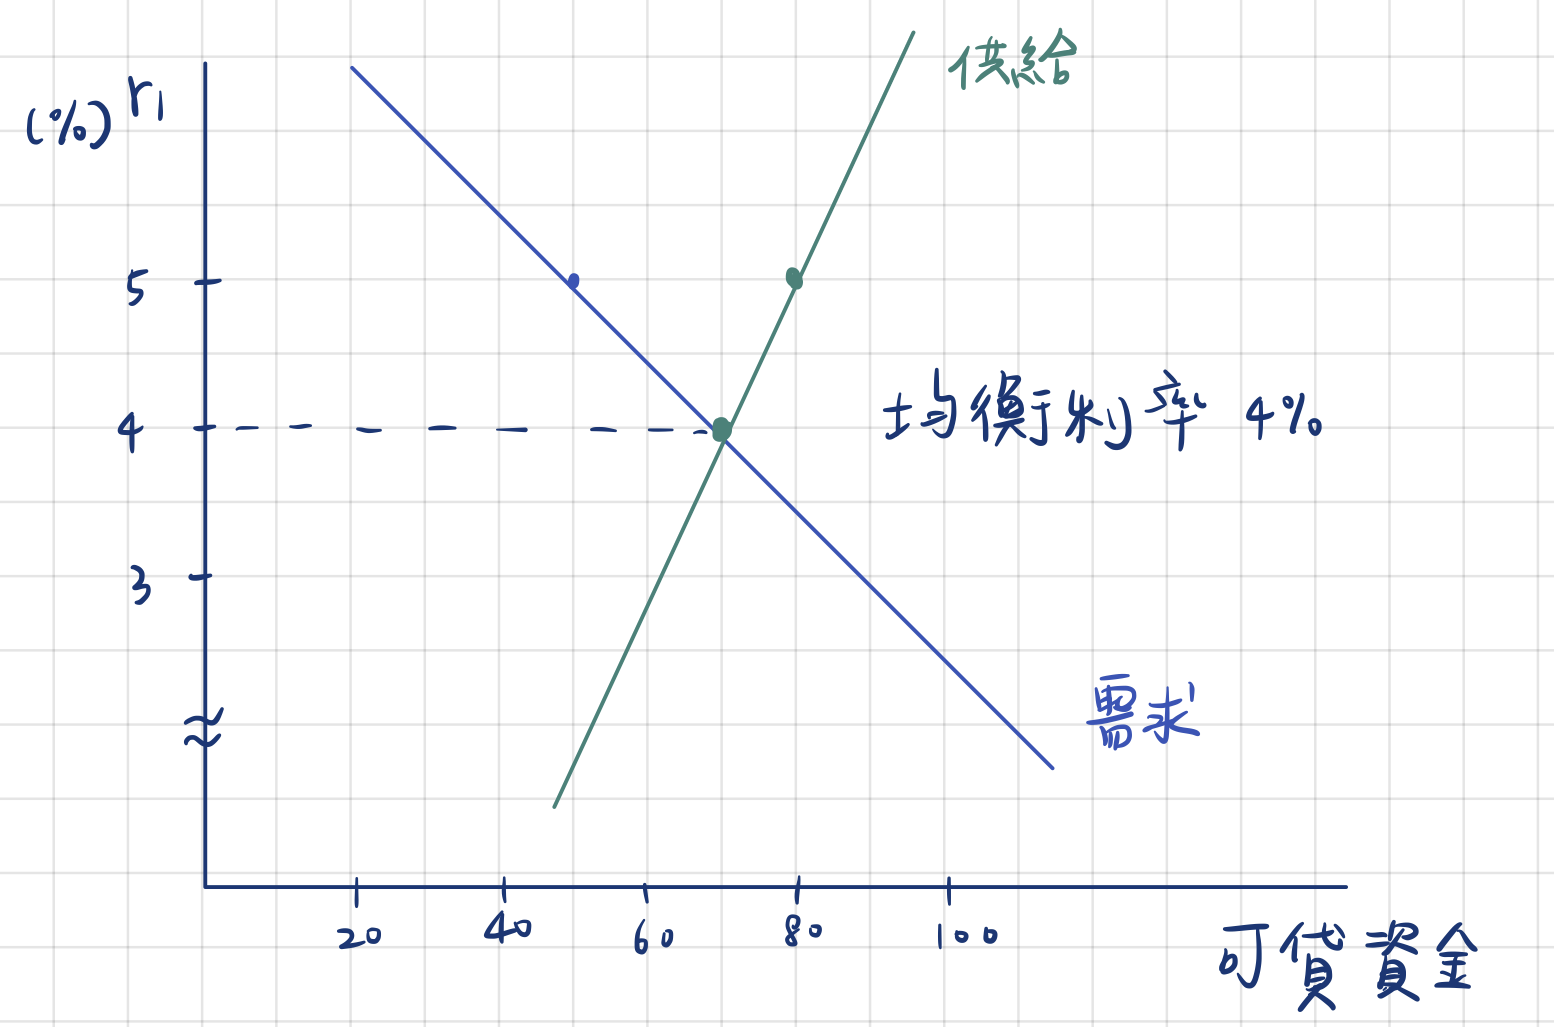
\includegraphics[scale = 0.25]{3a.png}
\end{figure}
\subsection{}
$$
\frac{B_1}{P_1} = S_1 - I_1 = 30
$$
\subsection{}
均衡利率會較高，借貸市場的供給線往左移$(S \to S')$

\begin{figure}[h]
    \centering
    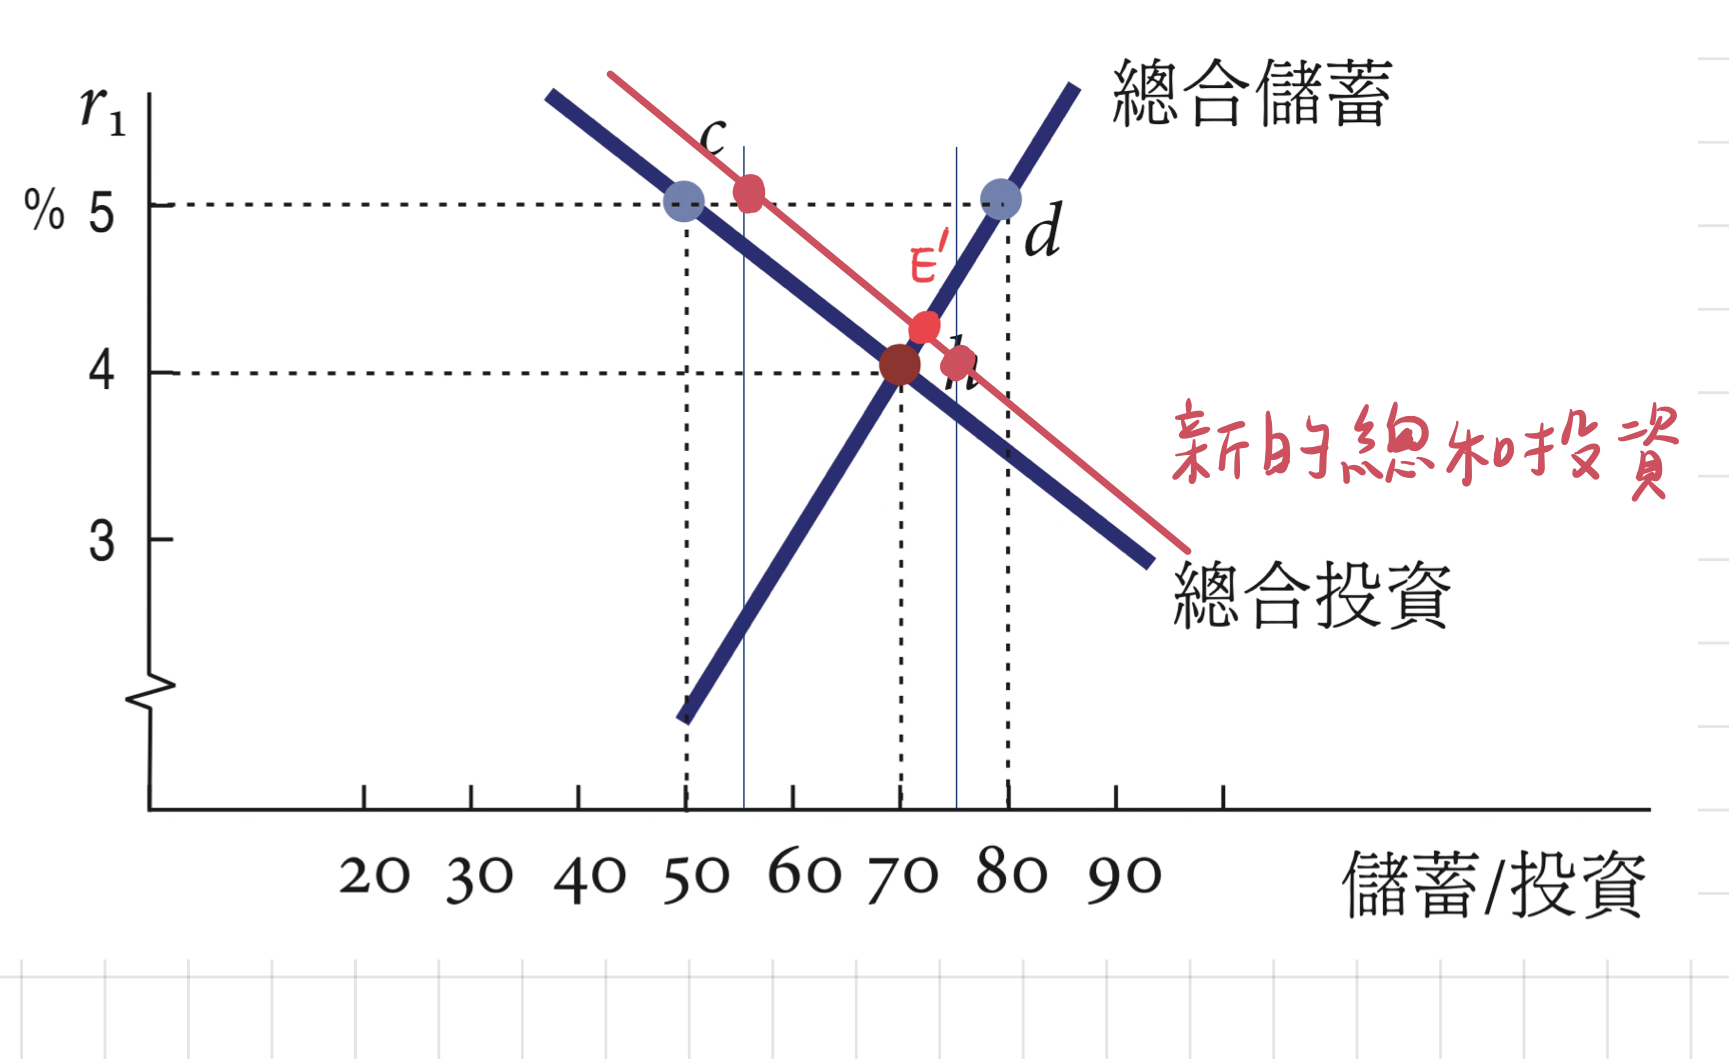
\includegraphics[scale = 0.15]{3c.png}
\end{figure}

\pagebreak
\begin{figure}[h]
    \centering
    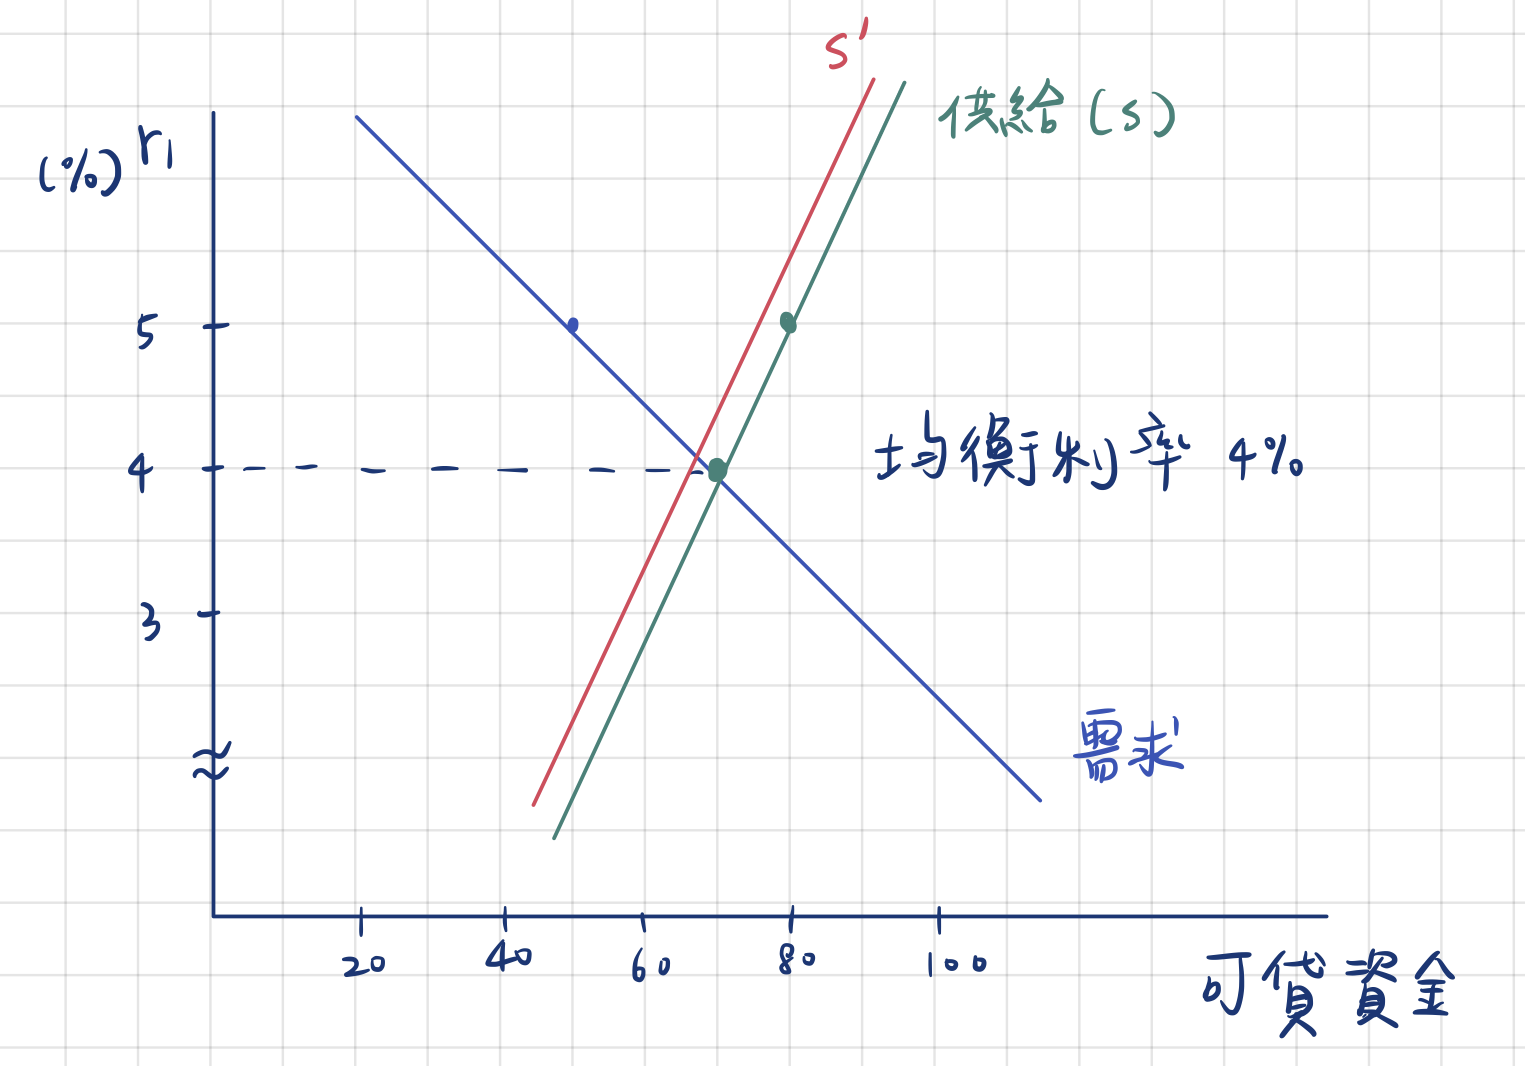
\includegraphics[scale = 0.2]{3c-2.png}
\end{figure}



\section{}
\begin{figure}[h]
    \centering
    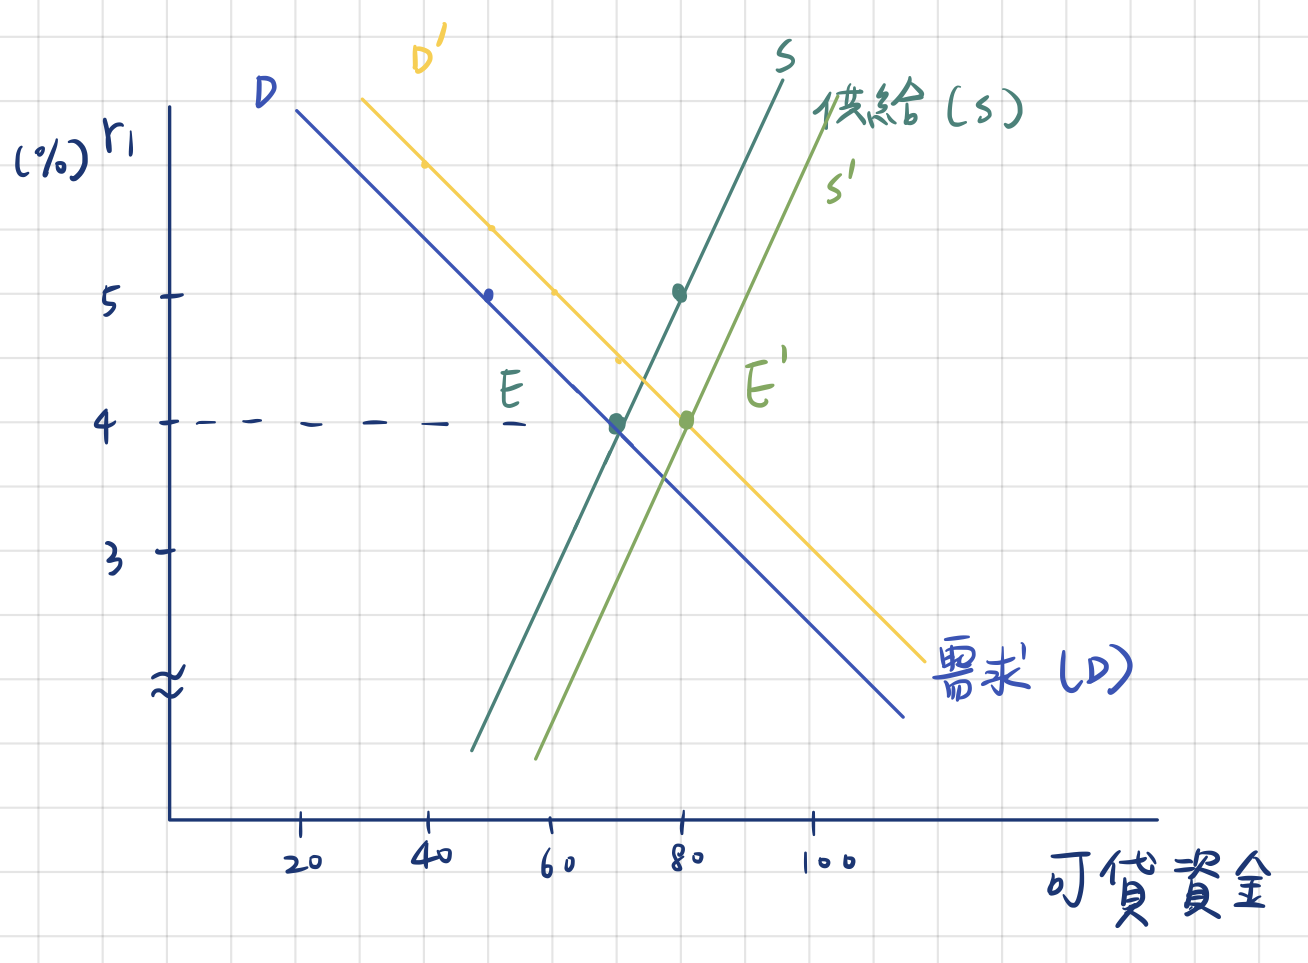
\includegraphics[scale = 0.25]{4.png}
\end{figure}

$$
D\to D' $$$$
S \to S'$$$$
E \to E'
$$

均衡利率不變，仍為 4\%

\section{}
\subsection{}
\begin{itemize}
    \item Generation Z: Born after 1997
    \item Baby-boomers: Born 1946 - 1964
\end{itemize}
\subsection{}
At least 5\%

\subsection{}
About 3\%. \\
\textbf{Quote} 
To do this, they assume that the real return on equities will be equal to the inflation-adjusted return on a risk-free asset (represented by Treasury bills), which they estimate at -0.5\%, plus a “risk premium” for buying equities of about 3.5\%, for a real return of just 3\%.

\subsection{}
Mr Marsh recommends adopting the time-honoured (if unexciting) principles of long-term investment, including \textbf{starting early}, \textbf{diversifying risk} and \textbf{avoiding high management fees.}

Rather than checking the value of their investments every ten minutes and trading frantically, they should exercise \textbf{patience} and sit out temporary shocks and turbulence.
\\ 由上述引文可知：及早準備、分散風險、避免高的管理費用（去買ETF），並且對股市的波動保持耐心是作者給予 Generation Z 在投資策略上的建議。

\subsection{}
The quick bounce back is rare in equity market, and we shouldn't concerned it as normal. That's why we are "lucky".
\end{document}


